\documentclass[aspectratio=169,11pt,hyperref={colorlinks=true}]{beamer}
\usetheme{boxes}
\setbeamertemplate{navigation symbols}{}
\definecolor{IBMblue}{RGB}{31,112,193}
\setbeamercolor{titlelike}{fg=IBMblue}
\setbeamercolor{structure}{fg=IBMblue}
\hypersetup{colorlinks,urlcolor=IBMblue}
\setbeamertemplate{footline}[frame number]
% Inserting graphics
\usepackage{graphicx}
% Side-by-side figures, etc
\usepackage{subfigure}
% Code snippits
\usepackage{listings}
\usepackage{minted}

\usepackage{lmodern}
% Color stuff
\usepackage{color}
\usepackage{amsmath}
\usepackage{tikz}
\usepackage{gensymb}
\newcommand\RBox[1]{%
  \tikz\node[draw,rounded corners,align=center,] {#1};%
}
\usepackage{hyperref}
%\usecolortheme{buzz}
%\usecolortheme{wolverine}
%\usetheme{Boadilla}
\usepackage[T1]{fontenc}

\definecolor{mygreen}{rgb}{0,0.6,0}
\definecolor{mygray}{rgb}{0.5,0.5,0.5}
\definecolor{mymauve}{rgb}{0.58,0,0.82}

\lstset{%
  backgroundcolor=\color{white},   % choose the background color; you must add \usepackage{color} or \usepackage{xcolor}
  breakatwhitespace=false,         % sets if automatic breaks should only happen at whitespace
  breaklines=true,                 % sets automatic line breaking
  captionpos=b,                    % sets the caption-position to bottom
  commentstyle=\color{IBMblue},  % comment style
  extendedchars=true,              % lets you use non-ASCII characters; for 8-bits encodings only, does not work with UTF-8
  keepspaces=true,                 % keeps spaces in text, useful for keeping indentation of code (possibly needs columns=flexible)
  keywordstyle=\color{blue},       % keyword style
%  otherkeywords={*,...},           % if you want to add more keywords to the set
  numbersep=5pt,                   % how far the line-numbers are from the code
  numberstyle=\tiny\color{mygray}, % the style that is used for the line-numbers
  rulecolor=\color{black},         % if not set, the frame-color may be changed on line-breaks within not-black text (e.g. comments (green here))
  showspaces=false,                % show spaces everywhere adding particular underscores; it overrides 'showstringspaces'
  showstringspaces=false,          % underline spaces within strings only
  showtabs=false,                  % show tabs within strings adding particular underscores
  stringstyle=\color{IBMblue},   % string literal style
}


\setbeamerfont{caption}{series=\normalfont,size=\fontsize{6}{8}}
\setbeamertemplate{caption}{\raggedright\insertcaption\par}

\setlength{\abovecaptionskip}{0pt}
\setlength{\floatsep}{0pt}

\author[Matthew Treinish]{%
    \texorpdfstring{%
        \centering
        Matthew Treinish\\
        Developer Advocate - IBM \\
        \href{mailto:mtreinish@kortar.org}{mtreinish@kortar.org}\\
        \texttt{mtreinish on Freenode}\\
        \href{https://github.com/mtreinish/intro-to-docker}{https://github.com/mtreinish/intro-to-docker}
   }
   {Matthew Treinish}
}
\date{July 9th, 2018}

\title{Introduction to Docker}
\begin{document}

\titlepage

\section{What is Docker?}
\begin{frame}
    \frametitle{What is Docker?}
    \begin{columns}[T]
        \begin{column}{.48\textwidth}
            \begin{itemize}
                \item Tooling and platform to manage containers
                \item Manages the lifecycle of containers
                \item Simplified interface on top of existing technologies for ease of use
                \item Works on linux, Mac OS X, and Windows
            \end{itemize}
        \end{column}
        \begin{column}{.48\textwidth}
            
\includegraphics[width=.9\textwidth]{Docker_logo.png}
        \end{column} 
    \end{columns}
\end{frame}

\begin{frame}
    \frametitle{Containers}
    \begin{itemize}
    \item A group of processes run in isolation
        \begin{itemize}
            \item Similar to VMs by managed at the process level
            \item Run on a shared kernel
        \end{itemize}
    \item Each container has its own namespaces
        \begin{itemize}
            \item \textbf{PID} process IDs
            \item \textbf{USER} user and group IDs
            \item \textbf{LTS} hostname and domain name
            \item \textbf{NS} mount points
            \item \textbf{NET} network devices, stacks, ports
            \item \textbf{IPC} inter-process communications, message queues
            \item \textbf{cgroups} controls limits and monitoring of resources
        \end{itemize}
    \end{itemize}
\end{frame}

\begin{frame}
    \frametitle{Containers vs VMs}
    \centering
    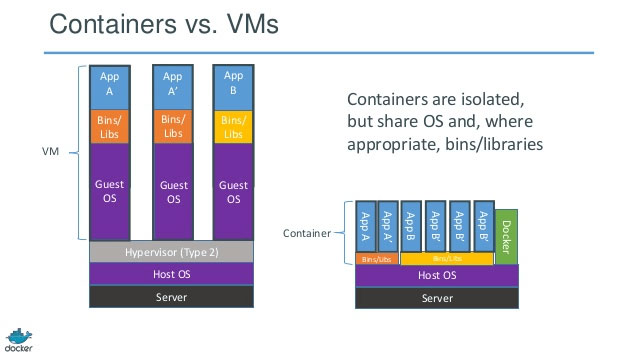
\includegraphics[width=.9\textwidth]{containers-vs-vm.jpg}
\end{frame}

\begin{frame}
    \frametitle{Why use containers?}
    \begin{itemize}
        \item Most of the same reasons as VMs (like isolation)
        \item Faster startup time, just the time to:
            \begin{itemize}
                \item Create new directory
                \item Setup the container's filesystem
                \item Setup network, mounts, etc
                \item Start the process
            \end{itemize}
        \item Better Resource utilization
        \item Reusability and distributability
    \end{itemize}
\end{frame}

\section{Getting Started with Docker}
\begin{frame}
    \frametitle{Installing Docker}
    \begin{itemize}
        \item On Linux - Distro Packages
        \item From Docker:
            \begin{itemize}
                \item Mac: \href{https://docs.docker.com/docker-for-mac/install/}{https://docs.docker.com/docker-for-mac/install/}
                \item Windows: \href{https://docs.docker.com/docker-for-windows/install/}{https://docs.docker.com/docker-for-windows/install/}
                \item Ubuntu: \href{https://docs.docker.com/v17.09/engine/installation/linux/docker-ce/ubuntu/}{https://docs.docker.com/v17.09/engine/installation/linux/docker-ce/ubuntu/}
            \end{itemize}
    \end{itemize}
\end{frame}

\subsection{Interacting with Docker}
\begin{frame}
    \frametitle{First container}
    {\LARGE \textbf{\$ docker run ubuntu echo Hello World}} \\
\end{frame}

\begin{frame}
    \frametitle{What Happened}
    \begin{itemize}
        \item Docker created a directory with an Ubuntu filesystem (image)
        \item Docker created a new set of namespaces
        \item Ran a new process: echo Hello World
        \item Using those namespaces to isolate it from other processes
        \item Using that new directory as the root of the filesystem (chroot)
        \item Notice as a user I never installed Ubuntu
        \item Run it again, notice how quickly it ran
    \end{itemize}
\end{frame}

\begin{frame}
    \frametitle{ssh-ing into a container}
    {\LARGE \textbf{\$ docker run -ti ubuntu bash}}
\end{frame}

\begin{frame}
    \frametitle{What Happened}
    \begin{itemize}
        \item Now the process is \textit{bash} instead of \textit{echo}
        \item But its still just a process
        \item Look around, mess around, its isolated
    \end{itemize}
\end{frame}

\begin{frame}
    \frametitle{Getting data into a container}
    \begin{itemize}
        \item Using env variables: \\
           \textbf{\$ docker run -e INPUT=IamSECURE -P ubuntu bash}
       \item Using Volumess: \\
           \textbf{\$ mkdir -p /tmp/volume \&\& echo IamSECURE > /tmp/volume/pass}\\
           \textbf{\$ docker run –i –t –v /tmp/volume:/volume ubuntu bash}
    \end{itemize}
\end{frame}

\begin{frame}
    \frametitle{Look under the covers}
    {\LARGE \textbf{\$ docker run ubuntu ps -ef}}
\end{frame}

\begin{frame}
    \frametitle{Things to notice with these examples}
    \begin{itemize}
        \item Each container only sees its own processes
        \item Running as root
        \item Running as PID 1
    \end{itemize}
\end{frame}


\section{Docker Images}
\begin{frame}
    \frametitle{Docker images}
    \begin{columns}[T]
        \begin{column}{.48\textwidth}
            \begin{itemize}
                \item Tarball of container's filesystem and metadata
                \item Makes sharing and distribution of containers easy
                \item Applications are packaged as images
            \end{itemize}
        \end{column}
        \begin{column}{.48\textwidth}
            \centering
            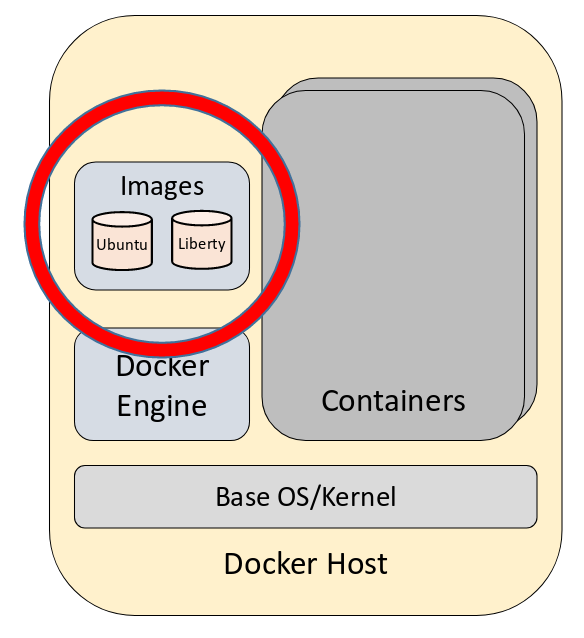
\includegraphics[width=.9\textwidth]{docker_images.png}
        \end{column}
    \end{columns}
\end{frame}

\begin{frame}
    \frametitle{Layering}
    \begin{columns}[T]
    \begin{column}{.48\textwidth}
        \begin{itemize}
            \item Docker uses a copy-on-write filesystem
            \item New files (or modifications) are only visible to current/above layers
            \item Layers allow for reuse
            \item Images are tarballs of layers
        \end{itemize}
    \end{column}
    \begin{column}{.48\textwidth}
        \centering
        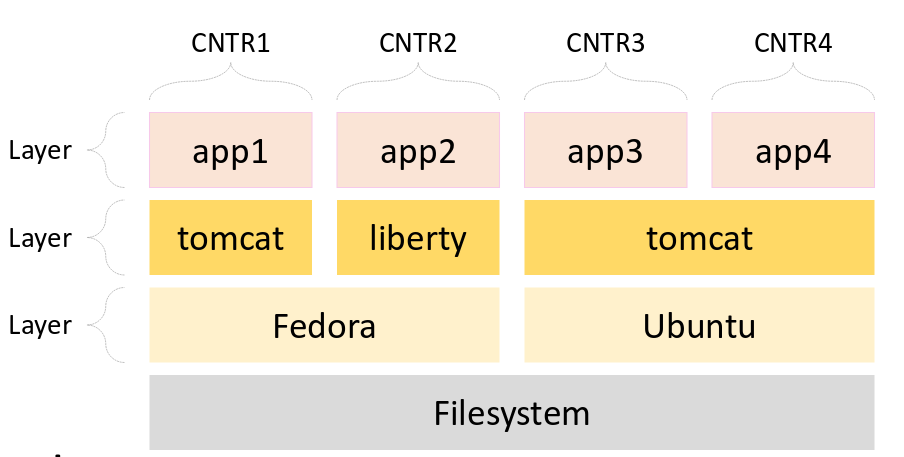
\includegraphics[width=\textwidth]{layering.png}
    \end{column}
    \end{columns}
\end{frame}

\begin{frame}
    \frametitle{Dockerhub}
    \href{https:/hub.docker.com}{https://hub.docker.com}
    \begin{itemize}
        \item Public registry of Docker Images
        \item Hosted by Docker Inc.
        \item Free for public images
        \item By default docker engines will look in DockerHub for images
        \item Browser interface for searching, descriptions of images
    \end{itemize}
\end{frame}

\begin{frame}
    \frametitle{Pick an application}
    Look at dockerhub and find a container for that application. \\ \\
    {\LARGE \textbf{\$ docker run nginx}}
\end{frame}

\begin{frame}
    \frametitle{What Happened}
    \begin{itemize}
        \item Pulled the nginx:latest image form dockerhub
            \begin{itemize}
                \item Dockerhub entry: \href{https://hub.docker.com/\_/nginx/}{https://hub.docker.com/\_/nginx/}
                \item Layered ontop of debian:stretch-slim image: \href{https://hub.docker.com/\_/debian/}{https://hub.docker.com/\_/debian/}
            \end{itemize}
        \item Run that container
        \item No configuration, just a base nginx
    \end{itemize}
\end{frame}

\begin{frame}
    \frametitle{Tie it all together}
    \textbf{\$ docker run -P -v examples/nginx/content:/usr/share/nginx/html:ro nginx}
\end{frame}

\subsection{Building Images}
\begin{frame}
    \frametitle{The Dockerfile}
    Reference Guide: \href{https://docs.docker.com/engine/reference/builder/}{https://docs.docker.com/engine/reference/builder/}
    \begin{itemize}
        \item Input script to build images
        \item Important instructions:
        \begin{itemize}
            \item \textbf{FROM} - Set base image either another Dockerfile or from a registry
            \item \textbf{RUN} - Run a command inside a new layer
            \item \textbf{COPY} - Copy files or directories into the filesystem of the container
            \item \textbf{CMD} - Set a default command for executing a container
            \item \textbf{EXPOSE} - Specify a port the container listens on
        \end{itemize}
    \end{itemize}
\end{frame}

\begin{frame}
    \frametitle{Example Dockerfile}
    \inputminted[fontsize=\small,breaklines,linenos,frame=single]{dockerfile}{examples/uwsgi/Dockerfile}
\end{frame}

\begin{frame}
    \frametitle{Building a Service image}
    \inputminted[fontsize=\scriptsize,breaklines,linenos,frame=single]{dockerfile}{examples/mosquitto/Dockerfile}
    \begin{itemize}
        \item \textbf{\$ docker build -t mymosquitto examples/mosquitto}
        \item \textbf{\$ docker run -e MQTT\_PASS=SecurePASS -P mymosquitto}
    \end{itemize}
\end{frame}


\begin{frame}
    \frametitle{Back to nginx}
    Build an image with the same content as our custom nginx before:
    \inputminted[fontsize=\large,breaklines,linenos,frame=single]{dockerfile}{examples/nginx/Dockerfile}
    \begin{itemize}
        \item {\large \textbf{\$ docker build -t mycustomhtml examples/nginx}}
        \item {\large \textbf{\$ docker run -P mycustomhtml}}
    \end{itemize}
\end{frame}

\begin{frame}
    \frametitle{What happened}
    \begin{itemize}
        \item Created a new image built on top of the nginx image from Docker Hub
        \item It copies the content directory into the nginx shared content directory
        \item Then run that image to get
    \end{itemize}

\end{frame}


\section{Image Registries}
\begin{frame}
    \frametitle{Running your own registry}
    {\Large \textbf{\$ docker run -d -p 5000:5000 \-\-name registry registry}}
\end{frame}

\begin{frame}
    \frametitle{What happened}
    \begin{itemize}
        \item Pulled the registry container from dockerhub
        \item Launched the container as a daemon (in the background)
        \item Maps localhost port 5000 to port 5000 on the container
    \end{itemize}
\end{frame}

\begin{frame}
    \frametitle{Using a Local Registry}
    \textbf{\$ docker pull debian} \\
    \textbf{\$ docker image tag debian localhost:5000/myspecialimage} \\
    \textbf{\$ docker push localhost:5000/myspecialimage} \\
    \textbf{\$ docker pull localhost:5000/myspecialimage}
\end{frame}

\begin{frame}
    \frametitle{What happened}
    \begin{itemize}
        \item Pulled the latest debian image from dockerhub
        \item Tagged that image off the local registry
        \item Push that tagged image to the local registry
        \item Pull that image from the registry to the local machine
    \end{itemize}
\end{frame}

\section{Conclusion}
\begin{frame}
    \frametitle{Conclusion}
    \begin{itemize}
        \item Docker provides a simple to use interface for containers
        \item Containers provide fast and lightweight isolation for applications
        \item Docker enables building packages that are easily deployable
        \item Large ecosystem of applications built for Docker
        \item Image layering makes it simple to build off of existing images
    \end{itemize}
\end{frame}

\subsection{Questions?}
\begin{frame}
\frametitle{Where to get more information}
    \begin{itemize}
        \item These Slides: \href{https://github.com/mtreinish/intro-to-docker}{https://github.com/mtreinish/intro-to-docker}
        \item Docker tutorial: \href{https://github.com/docker/labs/tree/master/beginner}{https://github.com/docker/labs/tree/master/beginner}
        \item Docker documentation: \href{https://docs.docker.com/}{https://docs.docker.com/}
        \item Best practice for Dockerfiles: \href{https://docs.docker.com/develop/develop-images/dockerfile\_best-practices/}{https://docs.docker.com/develop/develop-images/dockerfile\_best-practices/}
    \end{itemize}
\end{frame}

\end{document}
